% CVPR 2026 Paper Template; see https://github.com/cvpr-org/author-kit

\documentclass[10pt,twocolumn,letterpaper]{article}

%%%%%%%%% PAPER TYPE  - PLEASE UPDATE FOR FINAL VERSION
\usepackage{cvpr}              % To produce the CAMERA-READY version

\usepackage{iftex}
\ifXeTeX
  \usepackage{fontspec}
  \setmainfont{TeX Gyre Termes}
\fi

\usepackage{microtype}

% ---- packages and macros added for this report ----
\usepackage{graphicx}
\usepackage{booktabs}
\usepackage{pifont}            % \ding{51} (check) / \ding{55} (cross)
\newcommand{\TODO}[1]{\textcolor{red}{[TODO: #1]}}
\newcommand{\noans}{\texttt{\textless no answer\textgreater}}

\definecolor{okgreen}{RGB}{0,128,0}
\definecolor{badred}{RGB}{200,0,0}
\newcommand{\good}[1]{\textcolor{okgreen}{#1}}
\newcommand{\bad}[1]{\textcolor{badred}{#1}}
% ---------------------------------------------------

\definecolor{cvprblue}{rgb}{0.21,0.49,0.74}
\usepackage[pagebackref,breaklinks,colorlinks,allcolors=cvprblue]{hyperref}

%%%%%%%%% PAPER ID  - PLEASE UPDATE
\def\paperID{*****} % *** Enter the Paper ID here
\def\confName{CVPR}
\def\confYear{2026}

%%%%%%%%% TITLE - PLEASE UPDATE
\title{Assignment 2: MLLM with LLaVA}

%%%%%%%%% AUTHORS - PLEASE UPDATE
\author{B12508026 TAI, WEI-HSUAN}

\begin{document}
\maketitle

%%%%%%%%% BODY TEXT

% ============================================================================ %
%                                   ABSTRACT                                   %
% ============================================================================ %

\begin{abstract}
We evaluate LLaVA-1.5-7B \cite{NEURIPS2023_6dcf277e,liu2023improvedllava,llavahf2023llava15_7b} across zero-shot benchmark performance, LLM-as-a-judge consistency, component-wise LoRA fine-tuning, and custom LVLM construction. On a 5-image, 10-question personal benchmark, LLaVA scored 6/10, matching Qwen2.5-VL-7B-Instruct (native preprocessing) \cite{bai2025qwen25vl,qwen25vl7b_hf}. Using GPT-6.1-Sol and GPT-6.1-Terra as judges \cite{openai2026gpt61sol_card,openai2026gpt61terra_card}, verdicts remained consistent across all ten order-swapped pairs, though both judges misjudged the same two items. Fine-tuning on ScreenQA Short \cite{hsiao2024screenqa} using language-only LoRA raised test EM/F1 from 25.8/34.4 to 37.9/49.6. Adding the projector and vision encoder yielded 37.7/49.8 and 40.0/51.6, respectively, within roughly one standard error. And all three configurations answered all ten personal questions identically. Finally, our custom LVLM (CLIP \cite{radford2021clip} + Qwen2.5-0.5B-Instruct \cite{qwen2025qwen25}) gained captioning and semantic QA capabilities after alignment and instruction tuning, but still struggled with OCR and counting.
\end{abstract}

% ============================================================================ %
%                              1. SETUP AND METHOD                             %
% ============================================================================ %

\section{Setup and Method}

\subsection{Environment Setting}

All experiments ran on one NVIDIA GeForce RTX 5070 Ti GPU (16\,GB VRAM, driver 570.211.01) with Python 3.12.15, PyTorch 2.8.0+cu128 (CUDA 12.8, cuDNN 9.10.2), Hugging Face Transformers 4.57.1 and PEFT 0.17.1 (Fig.~\ref{Fig:env}). Figures were drawn in a separate environment with matplotlib 3.10.6, and training curves were logged with TensorBoard 2.20.0. 

\begin{figure}[t]
  \centering
  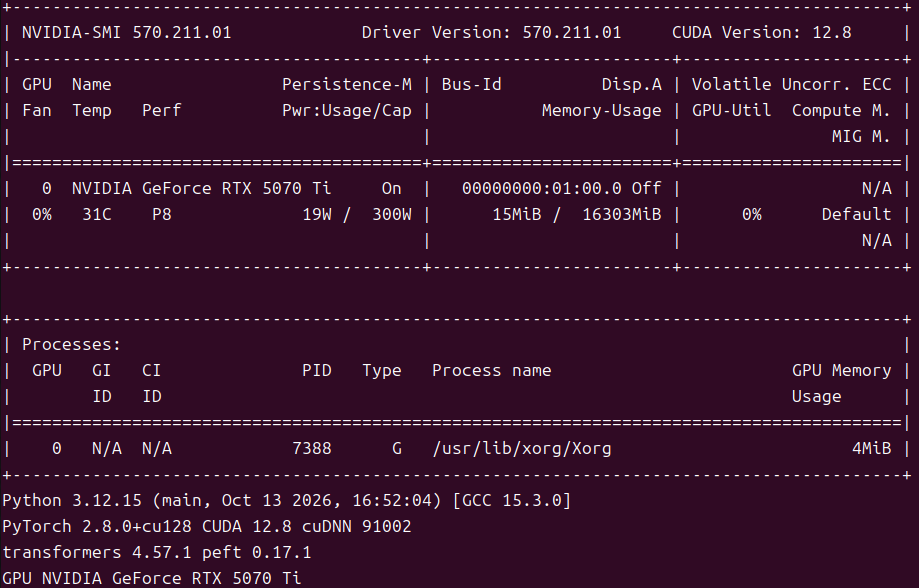
\includegraphics[width=\linewidth]{src/environment.png}
  \caption{Experimental environment (\texttt{nvidia-smi} and library versions).}
  \label{Fig:env}
\end{figure}

\subsection{Codebase Structure Description}

This is a brief description of the codebase, see \texttt{README.md} for details.

\begin{itemize}
  \item \texttt{train.py}: the main entry of LoRA training.
  \item \texttt{evaluate.py}: scores saved checkpoints on a panel (EM/F1);
        \texttt{summarize.py} exports \texttt{comparison.csv} and curves.
  \item \texttt{studies/}: personal images and questions with expected answers.
  \item \texttt{comparison.py}, \texttt{llm\_judge/judge.py}: second LVLM (Qwen2.5-VL-7B) and the API judge.
  \item \texttt{summarize.py}: exports \texttt{comparison.csv} and curves.
  \item \texttt{A\_plus/}: own LVLM construction; entry \texttt{run.sh}.
  \item \texttt{report/}: Raw results collected from separate \texttt{.jsonl} files and organized using Claude Code. Claude Code was strictly limited to file organization, and any automated analysis was forbidden.
\end{itemize}


\subsection{Fine-Tuning Protocol}

All three adapted models follow the fixed course recipe (Tab.~\ref{tab:recipe}). Each starts independently from the Original LLaVA weights with the same seed, data order, LoRA initialization, prompt and update budget; no model continues from an earlier variant. The loss is computed only on the first reference answer (\texttt{ground\_truth[0]}) plus EOS, with prompt, image and padding tokens masked. Generated answers are scored against \emph{all} references with the official normalized EM and F1. We report the prescribed final checkpoint (step 500) as the primary result; checkpoints 0 and 250 are only used for curves.

\begin{table}[t]
  \centering
  \small
  \begin{tabular}{@{}p{.27\columnwidth}p{.68\columnwidth}@{}}
    \toprule
    Setting & Value \\
    \midrule
    Start / duration & Original LLaVA; 1 epoch = 500 updates \\
    Batch            & microbatch 1 $\times$ accumulation 8 \\
    Optimizer        & AdamW, LR $2\times10^{-4}$, 5 warmup steps, cosine \\
    Regularization   & grad clip 1.0, no weight decay \\
    LoRA             & rank 8, $\alpha=16$, dropout 0~\cite{hu2022lora} \\
    Seed             & 17 \\
    Input            & square-padded to 336\,px (CLIP mean) \\
    Max sequence     & 1024 tokens \\
    Evaluation       & greedy, $\le$64 new tokens, step 500 \\
    \bottomrule
  \end{tabular}
  \caption{Fixed fine-tuning recipe, identical for all three scopes.}
  \label{tab:recipe}
\end{table}

\subsection{Component Scopes}

We compare three LoRA scopes, all with the vision encoder, projector and LLM base weights frozen:
\begin{itemize}
  \item \textbf{Language}: LoRA on the q/k/v/o projections of all 32 LLM layers, $4 \times 8 \times (4096+4096) \times 32 = 8{,}388{,}608$ parameters.
  \item \textbf{+ Projector}: additionally LoRA on both projector linears, $8 \times (1024+4096) + 8 \times (4096+4096) = 106{,}496$ parameters.
  \item \textbf{+ Vision}: additionally LoRA on the q/k/v/out projections of CLIP blocks 19--22, $4 \times 8 \times (1024+1024) \times 4 = 262{,}144$ parameters.
\end{itemize}
Tab.~\ref{tab:params} lists the counts per part; every part a scope claims to adapt is nonzero. We verified the hooks by checking that, after the first backward pass, the adapted parts receive nonzero gradients (e.g., \ projector \texttt{linear\_2} LoRA-B norm 0.052; vision blocks 19--22 \texttt{out\_proj} LoRA-B norms 0.036--0.050), that all sampled LoRA-B elements change during training, and that the base weights stay frozen. Because LoRA-B is initialized to zero, step 0 reproduces the Original model exactly: its validation and test scores match the Original's to every digit, and the first two training losses (2.1937, 1.8026) are identical across scopes.

\begin{table}[t]
  \centering
  \small
  \setlength{\tabcolsep}{4pt}
  \begin{tabular}{lrrrrr}
    \toprule
    Scope & Language & Projector & Vision & Total & Share \\
    \midrule
    Language     & 8,388,608 & 0       & 0       & 8,388,608 & 0.119\% \\
    + Projector  & 8,388,608 & 106,496 & 0       & 8,495,104 & 0.120\% \\
    + Vision     & 8,388,608 & 106,496 & 262,144 & 8,757,248 & 0.124\% \\
    \bottomrule
  \end{tabular}
  \caption{Trainable LoRA parameters per part. Share is relative to the 7,063,427,072 ($\approx$7B) parameters of the base model (language 6.74B, projector 21.0M, vision 303.5M).}
  \label{tab:params}
\end{table}

\subsection{Models and Datasets}

\paragraph{Models.} The base model is LLaVA-1.5-7B\cite{llavahf2023llava15_7b} (\texttt{llava-hf/llava-1.5-7b-hf}, revision \texttt{b234b80}). It feeds a CLIP ViT-L/14 encoder~\cite{radford2021clip} at $336\times336$ px through a two-layer MLP projector into Vicuna-7B~\cite{vicuna2023}, so each image becomes 576 visual tokens. The comparison model for the judge study is Qwen2.5-VL-7B-Instruct~\cite{bai2025qwen25vl} (revision \texttt{cc59489}); to fit in 16\,GB its LLM is quantized to 4-bit NF4, while the vision tower stays in bf16. The judges are GPT-6.1-terra and GPT-6.1-sol, accessed via the OpenAI API on 2026-11-11. Our own LVLM (Sec.~\ref{sec:build}) combines CLIP ViT-L/14-336 with Qwen2.5-0.5B-Instruct~\cite{qwen2025qwen25}.

\paragraph{Datasets.} The personal benchmark has five images with two questions each (Sec.~\ref{sec:own}).
Fine-tuning uses ScreenQA Short~\cite{hsiao2024screenqa,screenqa_dataset}, where a
screenshot and a question map to a short answer or \noans; the screenshots come
from Rico~\cite{10.1145/3126594.3126651}. Only pixels and the question are given, with no OCR, UI hierarchy or answer boxes. Tab.~\ref{tab:splits} lists the supplied splits. Our own LVLM is trained on LLaVA-CC3M-Pretrain-595K~\cite{sharma2018cc3m} for alignment and on LLaVA-Instruct-150K with COCO train2017 images~\cite{lin2014coco} for instruction tuning~\cite{NEURIPS2023_6dcf277e}.

\begin{table}[t]
  \centering
  \small
  \begin{tabular}{lrrl}
    \toprule
    Split & Questions & Screenshots & Use \\
    \midrule
    Train (D4000)          & 4,000 & 4,000 & training, final eval \\
    \quad T128 probe       & 128   & --    & training probe \\
    Validation (V\_NEW512) & 512   & 467   & validation \\
    Test (T\_AUDIT512)     & 512   & 480   & final test \\
    \bottomrule
  \end{tabular}
  \caption{ScreenQA Short splits. T128 is a fixed subset of D4000, evaluated at checkpoints 0/250/500 to track training; ``Train'' results below are the full D4000 at step 500.}
  \label{tab:splits}
\end{table}

% ============================================================================ %
%                    2. OWN-IMAGE EXPLORATION AND JUDGING                      %
% ============================================================================ %

\section{Own-Image Exploration and Judging}
\label{sec:own}

\subsection{Zero-Shot Exploration}

We collected five images (Fig.~\ref{fig:own}): a desktop game (a), the McDonald's app (b) and Instagram (c) are screenshots; a baseball game (d) and a dinner table (e) are photos. The ten questions mix OCR, counting, visual state, semantics and spatial reasoning, and the expected answer and its visible evidence were recorded before inference. LLaVA used the benchmark prompt (\emph{``Answer the question about the screenshot with a short answer. If it cannot be answered from the screenshot, answer exactly \noans.''}), CLIP-mean square padding to 336\,px and greedy decoding (Tab.~\ref{tab:own}).

\begin{figure*}[t]
  \centering
  \begin{minipage}[b]{0.22\linewidth}\centering
    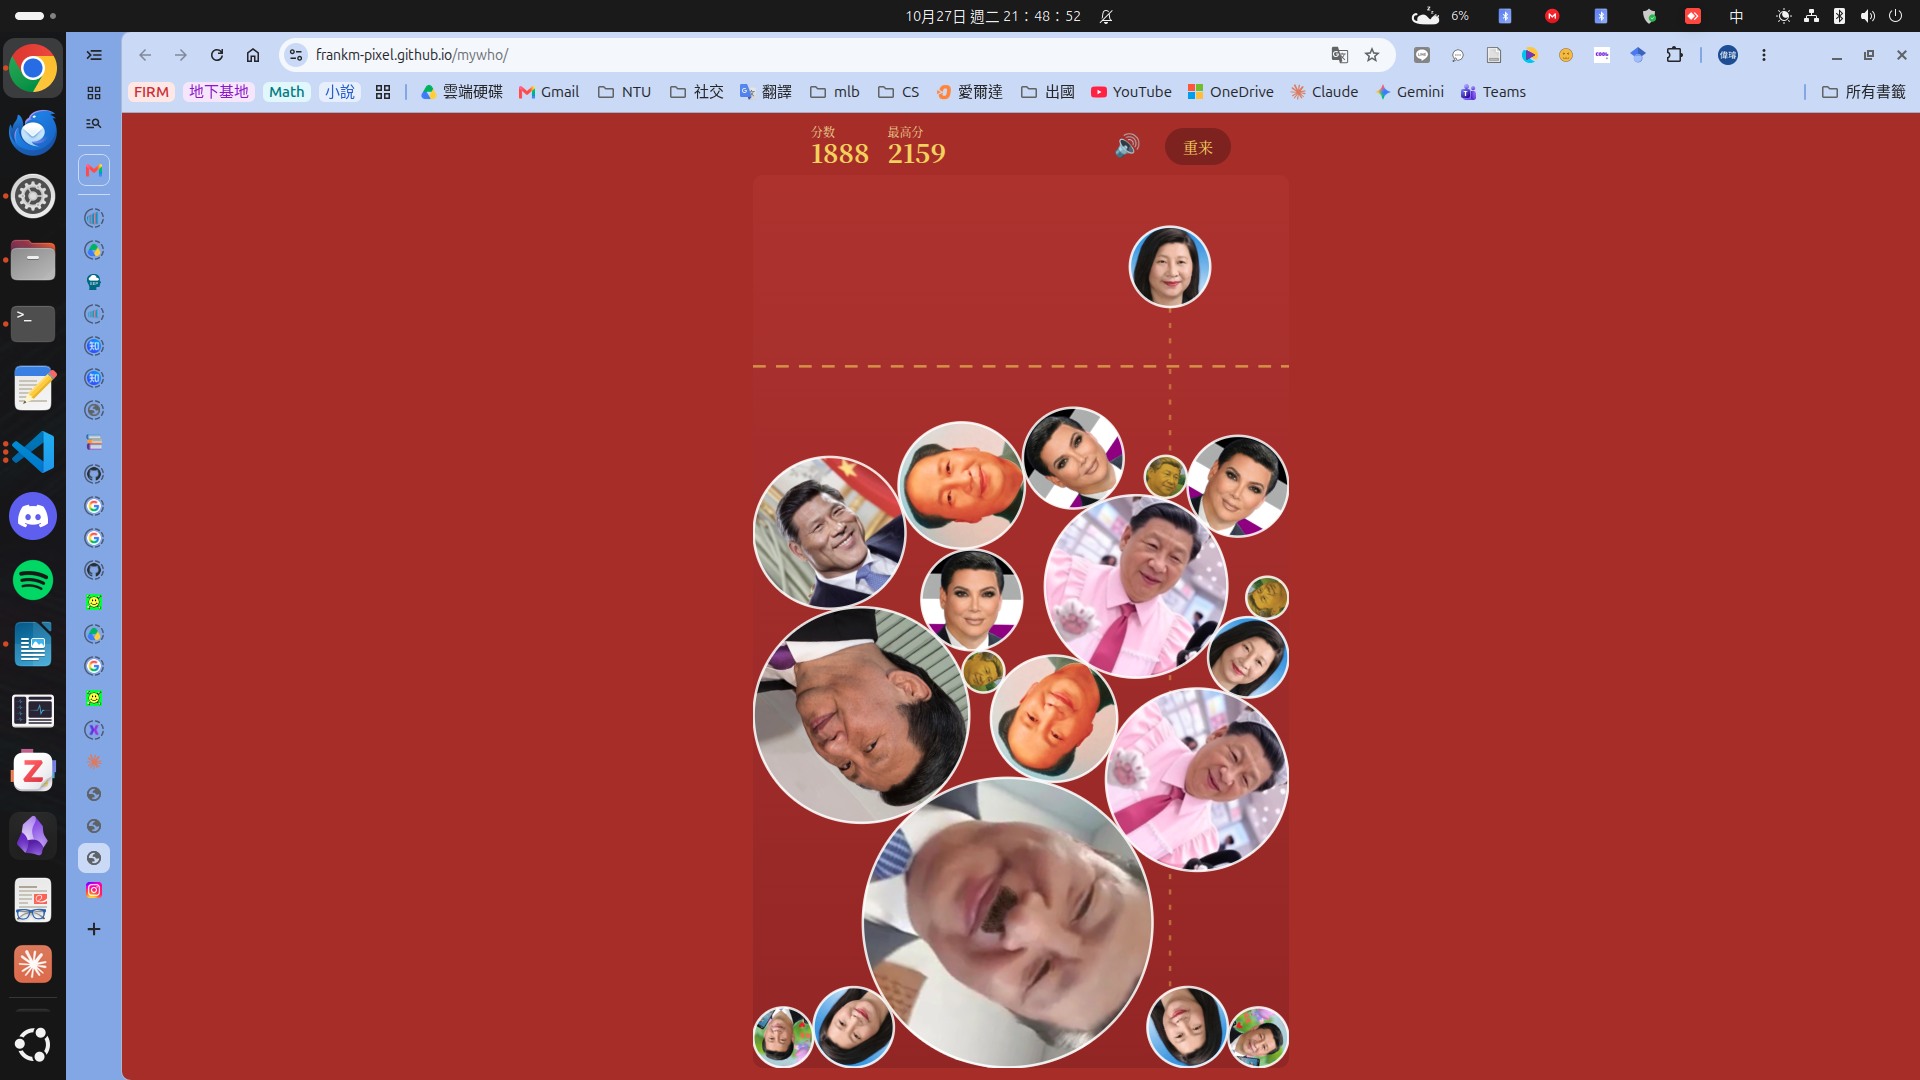
\includegraphics[width=\linewidth]{src/personal/a.png}\\(a) desktop game\end{minipage}\hfill
  \begin{minipage}[b]{0.13\linewidth}\centering
    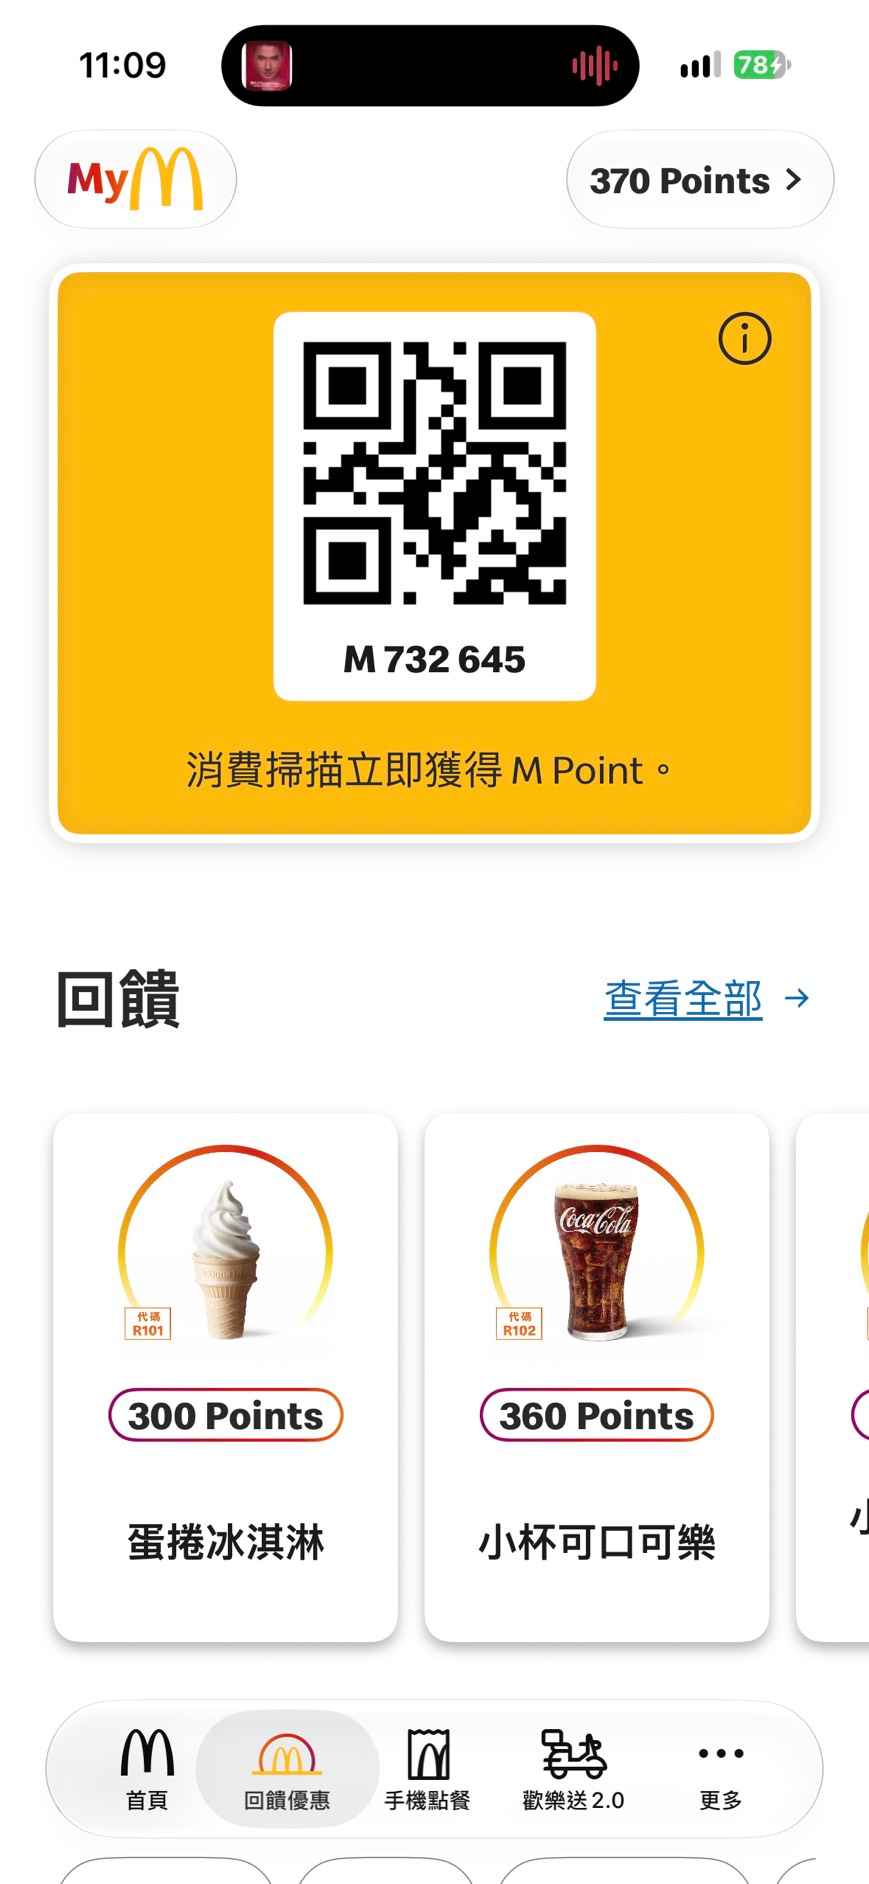
\includegraphics[width=\linewidth]{src/personal/b.png}\\(b) McDonald's app\end{minipage}\hfill
  \begin{minipage}[b]{0.13\linewidth}\centering
    
\includegraphics[width=\linewidth]{src/personal/c.png}\\(c) Instagram\end{minipage}\hfill
  \begin{minipage}[b]{0.22\linewidth}\centering
    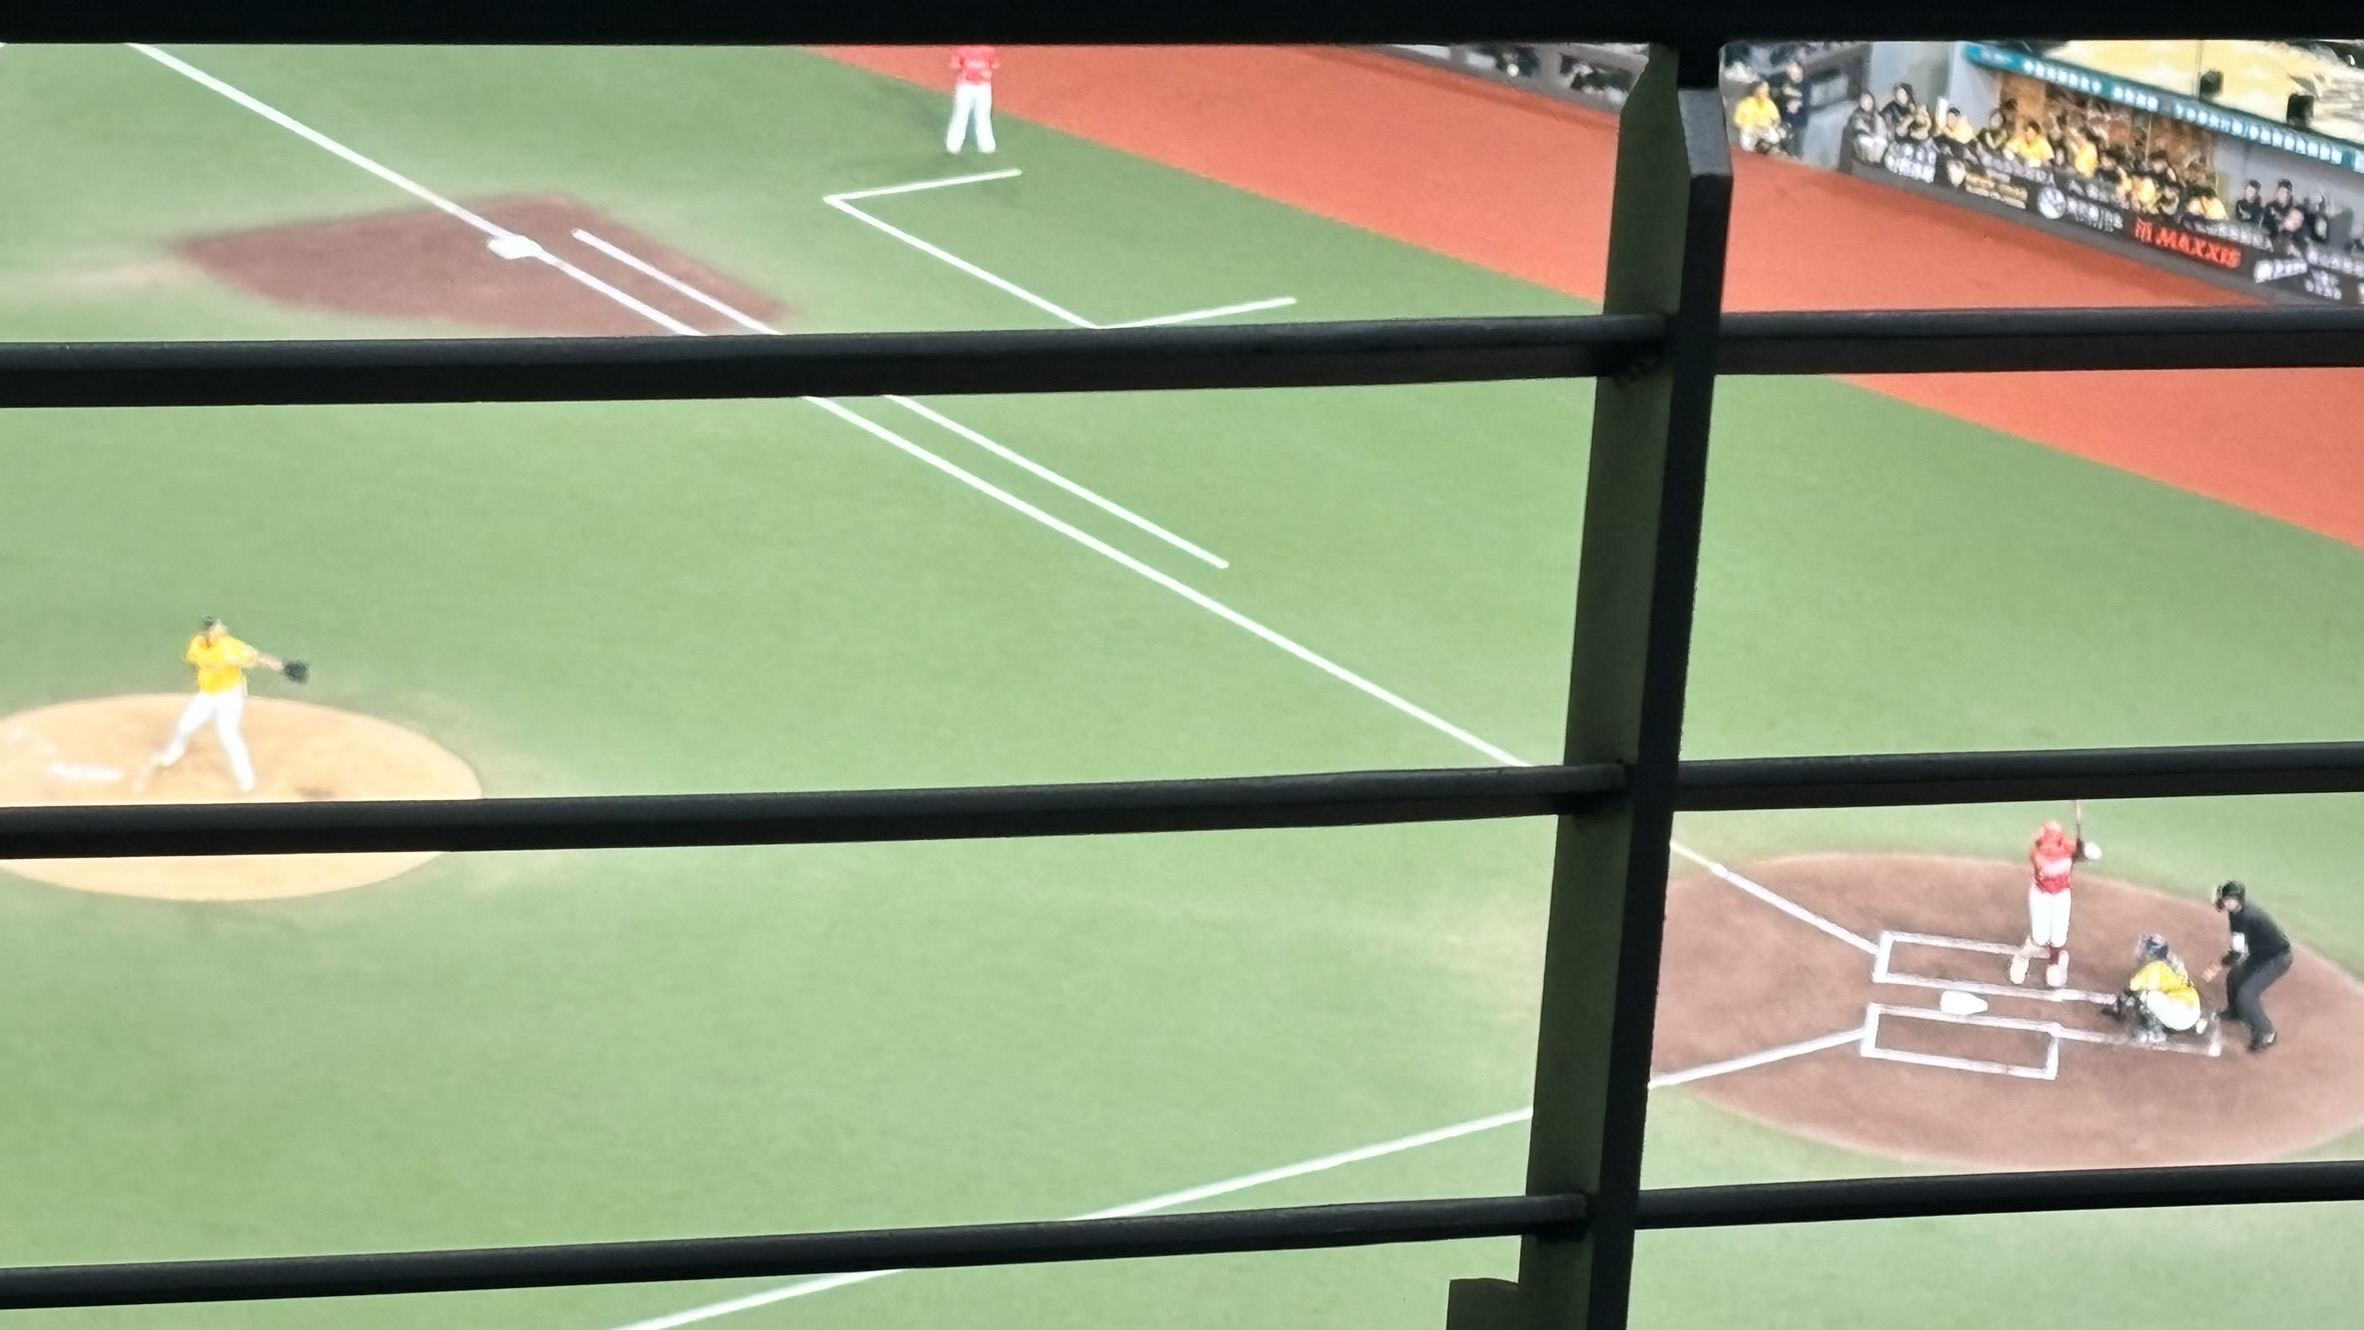
\includegraphics[width=\linewidth]{src/personal/d.png}\\(d) baseball\end{minipage}\hfill
  \begin{minipage}[b]{0.22\linewidth}\centering
    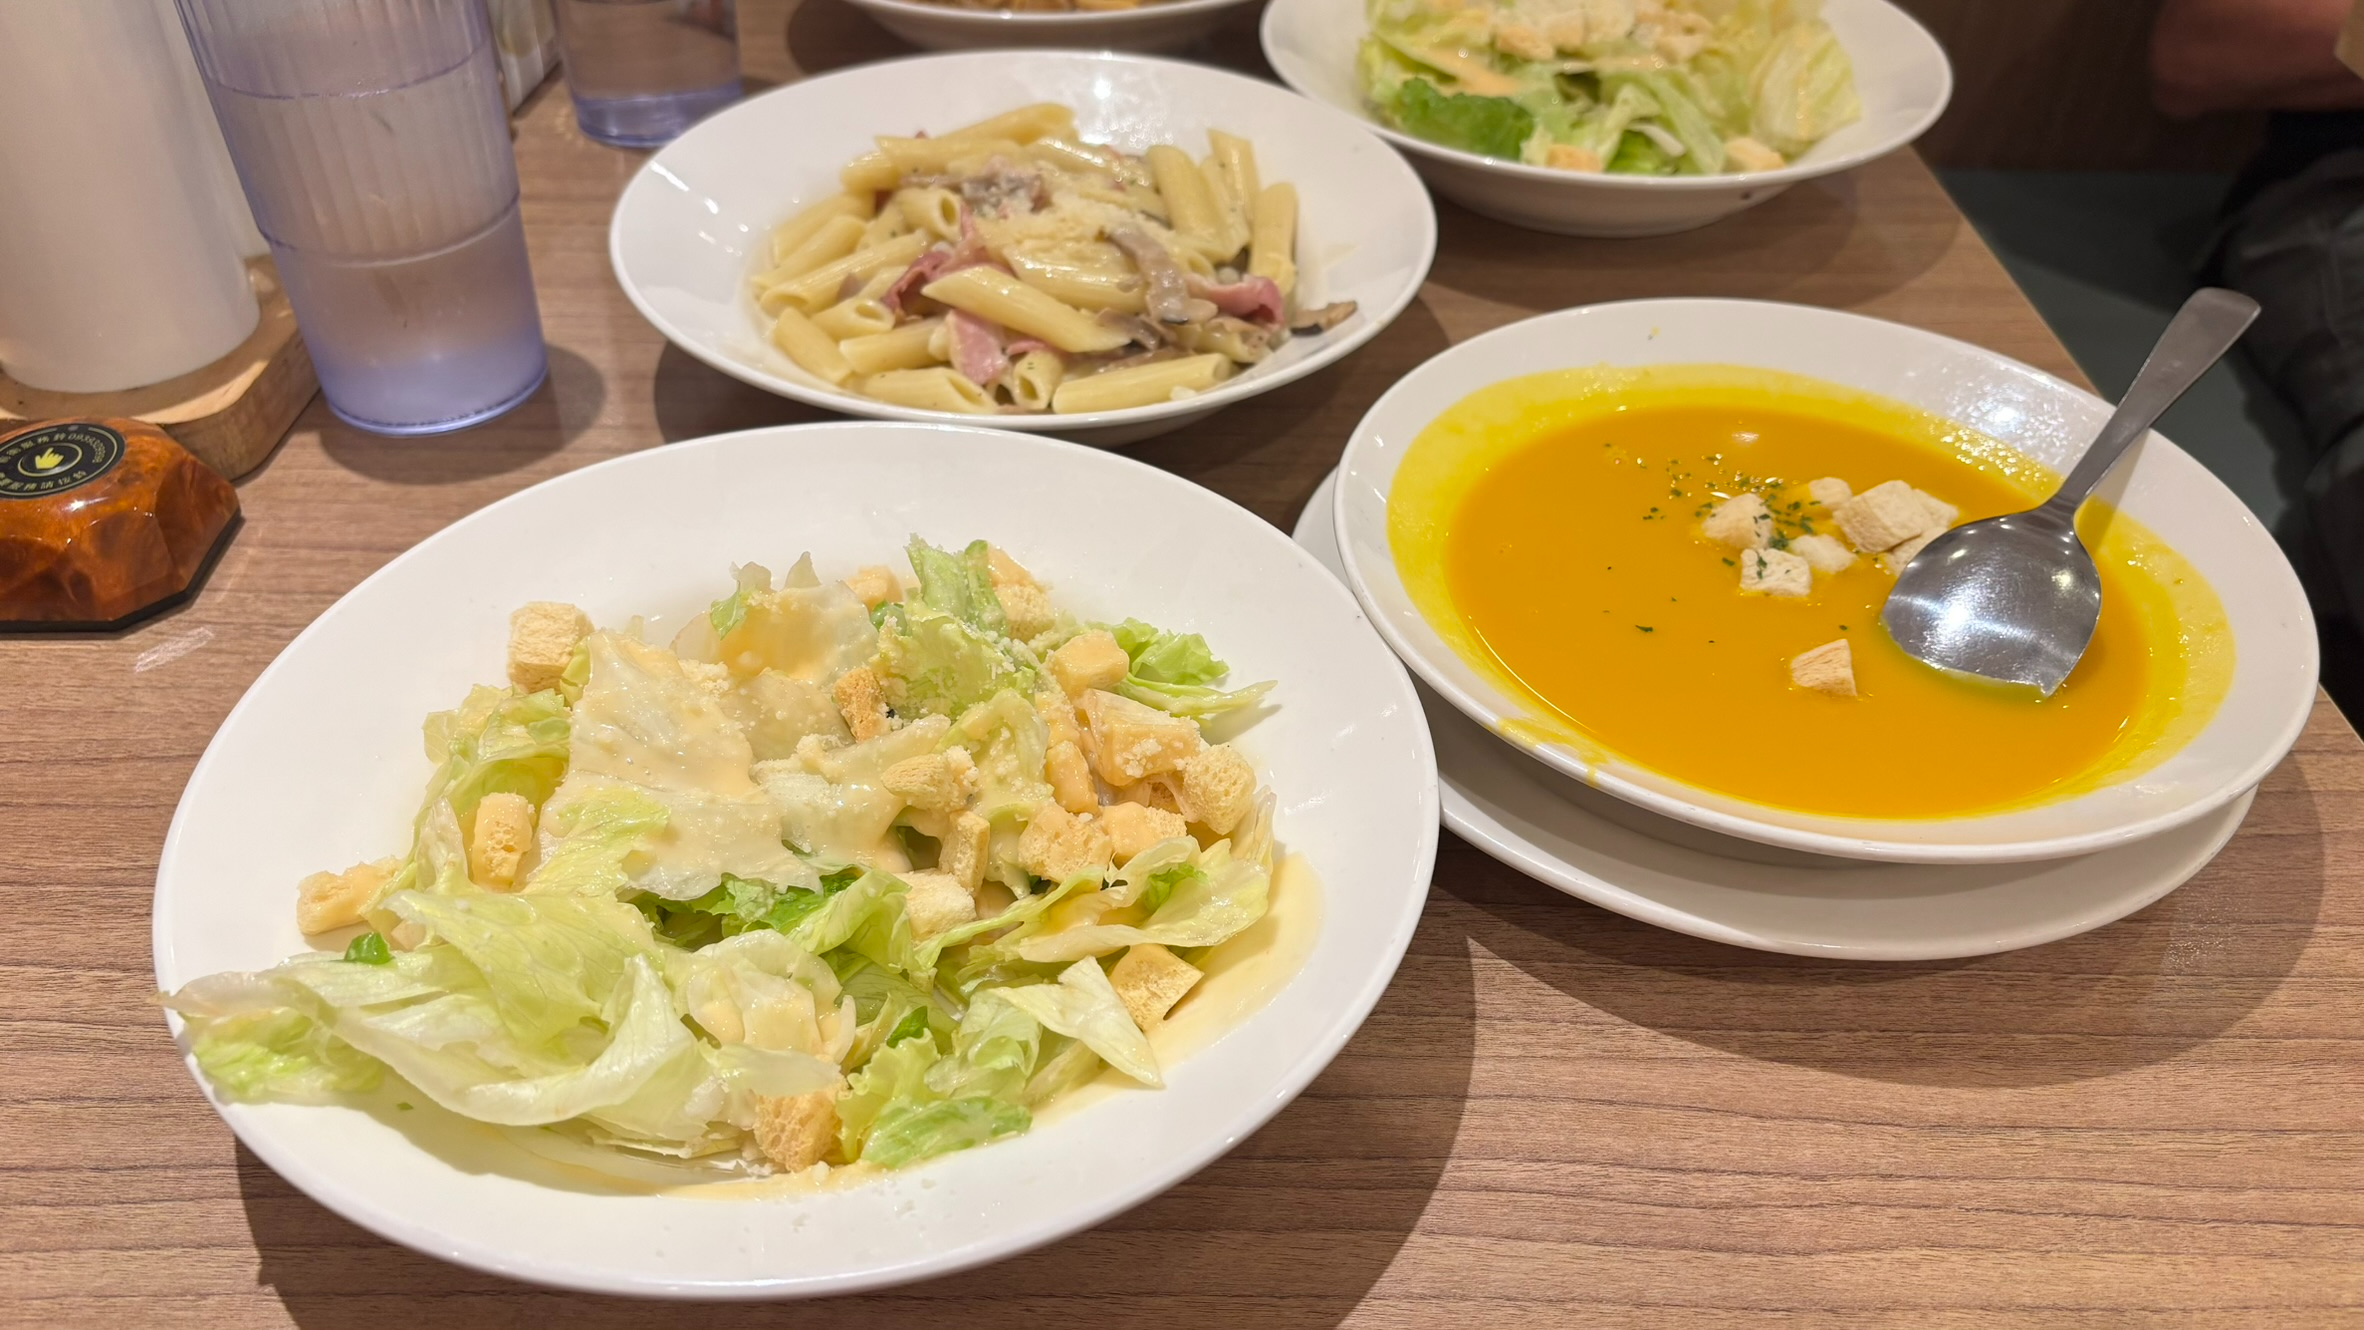
\includegraphics[width=\linewidth]{src/personal/e.png}\\(e) dinner table\end{minipage}
  \caption{The five personal images; (a)--(c) are screenshots, (d)--(e) are photos.}
  \label{fig:own}
\end{figure*}

\begin{table*}[t]
  \centering
  \footnotesize
  \setlength{\tabcolsep}{4pt}
  \begin{tabular}{llllll}
    \toprule
    ID & Fig. & Question & Expected (visible evidence) & LLaVA & Observation \\
    \midrule
    01-q1 & \ref{fig:own}a & Balls above the dashed line?    & 1 (lone ball above line)        & \bad{10}          & counts the pile, ignores the line \\
    01-q2 & \ref{fig:own}a & First icon in the left dock?    & Chrome (tricolor logo)          & \good{Chrome}     & logo recognized \\
    02-q1 & \ref{fig:own}b & Which company's app?            & McDonald's (golden M)           & \good{Mcdonald's} & brand recognized \\
    02-q2 & \ref{fig:own}b & Points left?                    & 370 (top-right balance)         & \bad{300}         & reads the larger reward cost \\
    03-q1 & \ref{fig:own}c & Author of the post?             & maths.cure (header handle)      & \bad{Maths Cure}  & reads the logo, not the handle \\
    03-q2 & \ref{fig:own}c & Am I following this account?    & No (button reads ``Follow'')    & \bad{Yes}         & misreads the button state \\
    04-q1 & \ref{fig:own}d & Players on the field?           & 3 (pitcher, batter, catcher)    & \good{3}          & excludes umpire and coach \\
    04-q2 & \ref{fig:own}d & Pitcher's jersey color?         & Yellow (pitcher on mound)       & \good{Yellow}     & ignores red distractors \\
    05-q1 & \ref{fig:own}e & Soup left/right of front salad? & Right (orange bowl)             & \good{Right}      & correct \\
    05-q2 & \ref{fig:own}e & How many salads?                & 2 (front left, back right)      & \good{2}          & correct \\
    \bottomrule
  \end{tabular}
  \caption{Zero-shot LLaVA-1.5-7B on the personal benchmark; answers in \good{green} are correct, in \bad{red} are wrong.}
  \label{tab:own}
\end{table*}

\paragraph{Failure analysis.} LLaVA correctly answers all four photo questions but only two of the six screenshot questions. Its successes share one property: the answer follows from large, salient, global features, such as a brand logo, a jersey color, the left/right layout of two bowls, or a count of two or three objects. Its four failures all require locating a small region and binding it to a constraint in the question:
(i) \emph{Counting under a spatial condition} (01-q1): it answers 10, roughly the size of the pile, ignoring the condition ``above the dashed line'' that leaves a single ball.
(ii) \emph{Salient distractor numbers} (02-q2): it picks 300, the largest number on the screen, which is a reward cost; our pre-recorded evidence note predicted exactly this confusion between a price and the user's balance.
(iii) \emph{Large text over small text} (03-q1): it reads the stylized ``MATHS Cure'' logo instead of the small header handle \texttt{maths.cure}.
(iv) \emph{UI state} (03-q2): it answers ``Yes'' although the button, labeled in Traditional Chinese, means ``Follow'' and thus implies the account is not followed; this requires both reading non-English UI text and knowing the convention.
LLaVA also never abstains: although the prompt allows \noans, it gives a definite answer to all ten questions, consistent with its 0/512 abstentions on the ScreenQA test (Sec.~\ref{sec:ft}). These errors are not simply a matter of input resolution: given the same $336\times336$ padded input, Qwen2.5-VL reads both the balance and the handle (Sec.~2.2). This points instead to LLaVA's CLIP encoder and training data, which target image--caption alignment rather than reading small screen text.


\subsection{LLM-as-a-Judge}
\label{sec:judge}

\paragraph{Setup.} The comparison model is Qwen2.5-VL-7B-Instruct~\cite{bai2025qwen25vl,qwen25vl7b_hf} (revision \texttt{cc59489}; LLM in 4-bit NF4, vision tower in bf16), which answers the same ten questions with the same prompt and greedy decoding. We first run it with its native preprocessing, which keeps the aspect ratio and allows up to 1,003,520 pixels, about $9\times$ the $336\times336=112{,}896$ pixels LLaVA sees. A difference between the two models could then come from the input rather than the model, so we also rerun Qwen with LLaVA's $336\times336$ square padding, giving both models identical pixels. Two judges evaluate both runs: GPT-6.1-Terra and GPT-6.1-Sol via the OpenAI API (model strings \texttt{gpt-6.1-terra} and \texttt{gpt-6.1-sol}; exact snapshots unknown), both accessed on 2026-11-11~\cite{zheng2023judging}. Each request contains the image, the question and anonymous Answers A/B, and asks for 0--5 scores, a verdict (A / B / tie / insufficient evidence) and a short visual justification. Both judges use identical prompts, temperature 0, seed 17, high image detail and a strict JSON schema. Each item is judged in both orders; every request is stateless, so each judgment is a fresh conversation.

\begin{table}[t]
  \centering
  \footnotesize
  \setlength{\tabcolsep}{3pt}
  \begin{tabular}{llccccc}
    \toprule
    Judge & Qwen input & LLaVA & Qwen & Tie & Insuff. & Score sums \\
    \midrule
    Terra & native & 1 & 2 & 7 & 0 & 30 / 35 \\
    Sol   & native & 1 & 2 & 7 & 0 & 30--32 / 35 \\
    Terra & 336 px & 1 & 1 & 8 & 0 & 34 / 34 \\
    Sol   & 336 px & 1 & 1 & 8 & 0 & 32--33 / 32--33 \\
    \midrule
    \multicolumn{2}{l}{Human labels (native / 336 px)} & \multicolumn{2}{c}{6 vs.\ 6 / 6 vs.\ 7} & & & \\
    \bottomrule
  \end{tabular}
  \caption{Judge verdicts, identical in both answer orders for every setting (winner kept on 10/10 swapped items). Score sums are LLaVA / Qwen over ten items (max 50); a range means the sum differs between the two orders.}
  \label{tab:judge}
\end{table}

\paragraph{One complete reply in each order (Terra, native, 02-q2).} Original order (A\,=\,LLaVA, B\,=\,Qwen):
{\small\begin{verbatim}
{"justification":"The balance at the top right
reads "370 Points." The 300 points shown below is
the cost of an ice cream reward.",
"score_A":0,"score_B":5,"verdict":"B"}
\end{verbatim}}
\noindent Reversed order (A\,=\,Qwen, B\,=\,LLaVA):
{\small\begin{verbatim}
{"justification":"The balance at the top right
reads "370 Points." The 300 points shown below is
the cost of an ice cream reward.",
"score_A":5,"score_B":0,"verdict":"A"}
\end{verbatim}}

\paragraph{Human disagreements.} We first use GPT-6.1-Terra alone, but it contradicts our pre-registered labels on two items. On 04-q1 it counts the red-uniformed base coach as a player, scoring LLaVA's correct ``3'' as 0 and Qwen's ``four'' as 5. On 03-q1 it accepts ``Maths Cure'' although our label requires the exact handle \texttt{maths.cure}. To test whether these errors are specific to Terra, we add GPT-6.1-Sol as a second judge, but it makes the same two mistakes; when Qwen also answers ``3'' under 336\,px input, Sol even scores both answers only 2--3 for ``undercounting''. Because both judges share these errors, they stem from an ambiguous item and a looser rubric rather than from one judge. As a result, although LLaVA and native Qwen both score 6/10 under our labels, both judges' score sums favor Qwen (Table~\ref{tab:judge}). With 336\,px input, three of Qwen's answers change (01-q2 becomes \noans, while 04-q1 and 05-q2 become correct), so the judges see a tie.

\paragraph{Is it a good metric?} Position bias barely affects the verdicts: both deterministic judges keep every winner when the order is swapped, although Sol's scores on 04-q1 shift with the order (0 vs.\ 2 and 2 vs.\ 3). Four weaknesses remain. (i) The judges make \emph{visual errors} (04-q1), so a verdict is bounded by the judge's perception, and a second judge from the same family does not fix them. (ii) They apply a \emph{looser rubric} than the task (03-q1). (iii) They score \emph{abstention} like a wrong answer, which matters because Qwen answers \noans{} on 3/10 items. (iv) Ties dominate (7--8/10), so the resolution is low on a small set. They do not favor length: full-sentence and one-word answers tie on 03-q1 and 05-q1. An LLM judge is a cheap relative signal, but it needs reference answers and a human audit of disagreements.

\section{Fine-Tuning Results}
\label{sec:ft}

\paragraph{Scores.} Tab.~\ref{tab:main} compares the Original model with the three scopes at step 500. On test, the three adaptations gain 12.1, 11.9 and 14.3 EM points. For T128 we report the Original as step 0, which is the same model.

\begin{table*}[t]
  \centering
  \small
  \begin{tabular}{lcccccccc}
    \toprule
    & \multicolumn{2}{c}{T128 probe ($n$=128)} & \multicolumn{2}{c}{Train D4000 ($n$=4,000)} & \multicolumn{2}{c}{Val ($n$=512 / 467 img)} & \multicolumn{2}{c}{Test ($n$=512 / 480 img)} \\
    \cmidrule(lr){2-3}\cmidrule(lr){4-5}\cmidrule(lr){6-7}\cmidrule(lr){8-9}
    Model & EM & F1 & EM & F1 & EM & F1 & EM & F1 \\
    \midrule
    Original LLaVA  & 31.25 & 38.45 & 25.47 & 34.21 & 26.56 & 35.29 & 25.78 & 34.38 \\
    Language LoRA   & 46.88 & 57.26 & 43.58 & 54.97 & 39.65 & 52.31 & 37.89 & 49.61 \\
    + Projector     & 46.09 & 57.55 & 43.92 & 55.15 & 39.65 & 52.61 & 37.70 & 49.77 \\
    + Vision        & \textbf{47.66} & \textbf{57.58} & \textbf{45.57} & \textbf{56.42} & \textbf{39.84} & \textbf{52.79} & \textbf{40.04} & \textbf{51.55} \\
    \bottomrule
  \end{tabular}
  \caption{ScreenQA Short EM/F1 (\%) at the final checkpoint (step 500). T128 is the training probe; ``Train'' is the full D4000 evaluation.}
  \label{tab:main}
\end{table*}

\begin{figure*}[t]
  \centering
  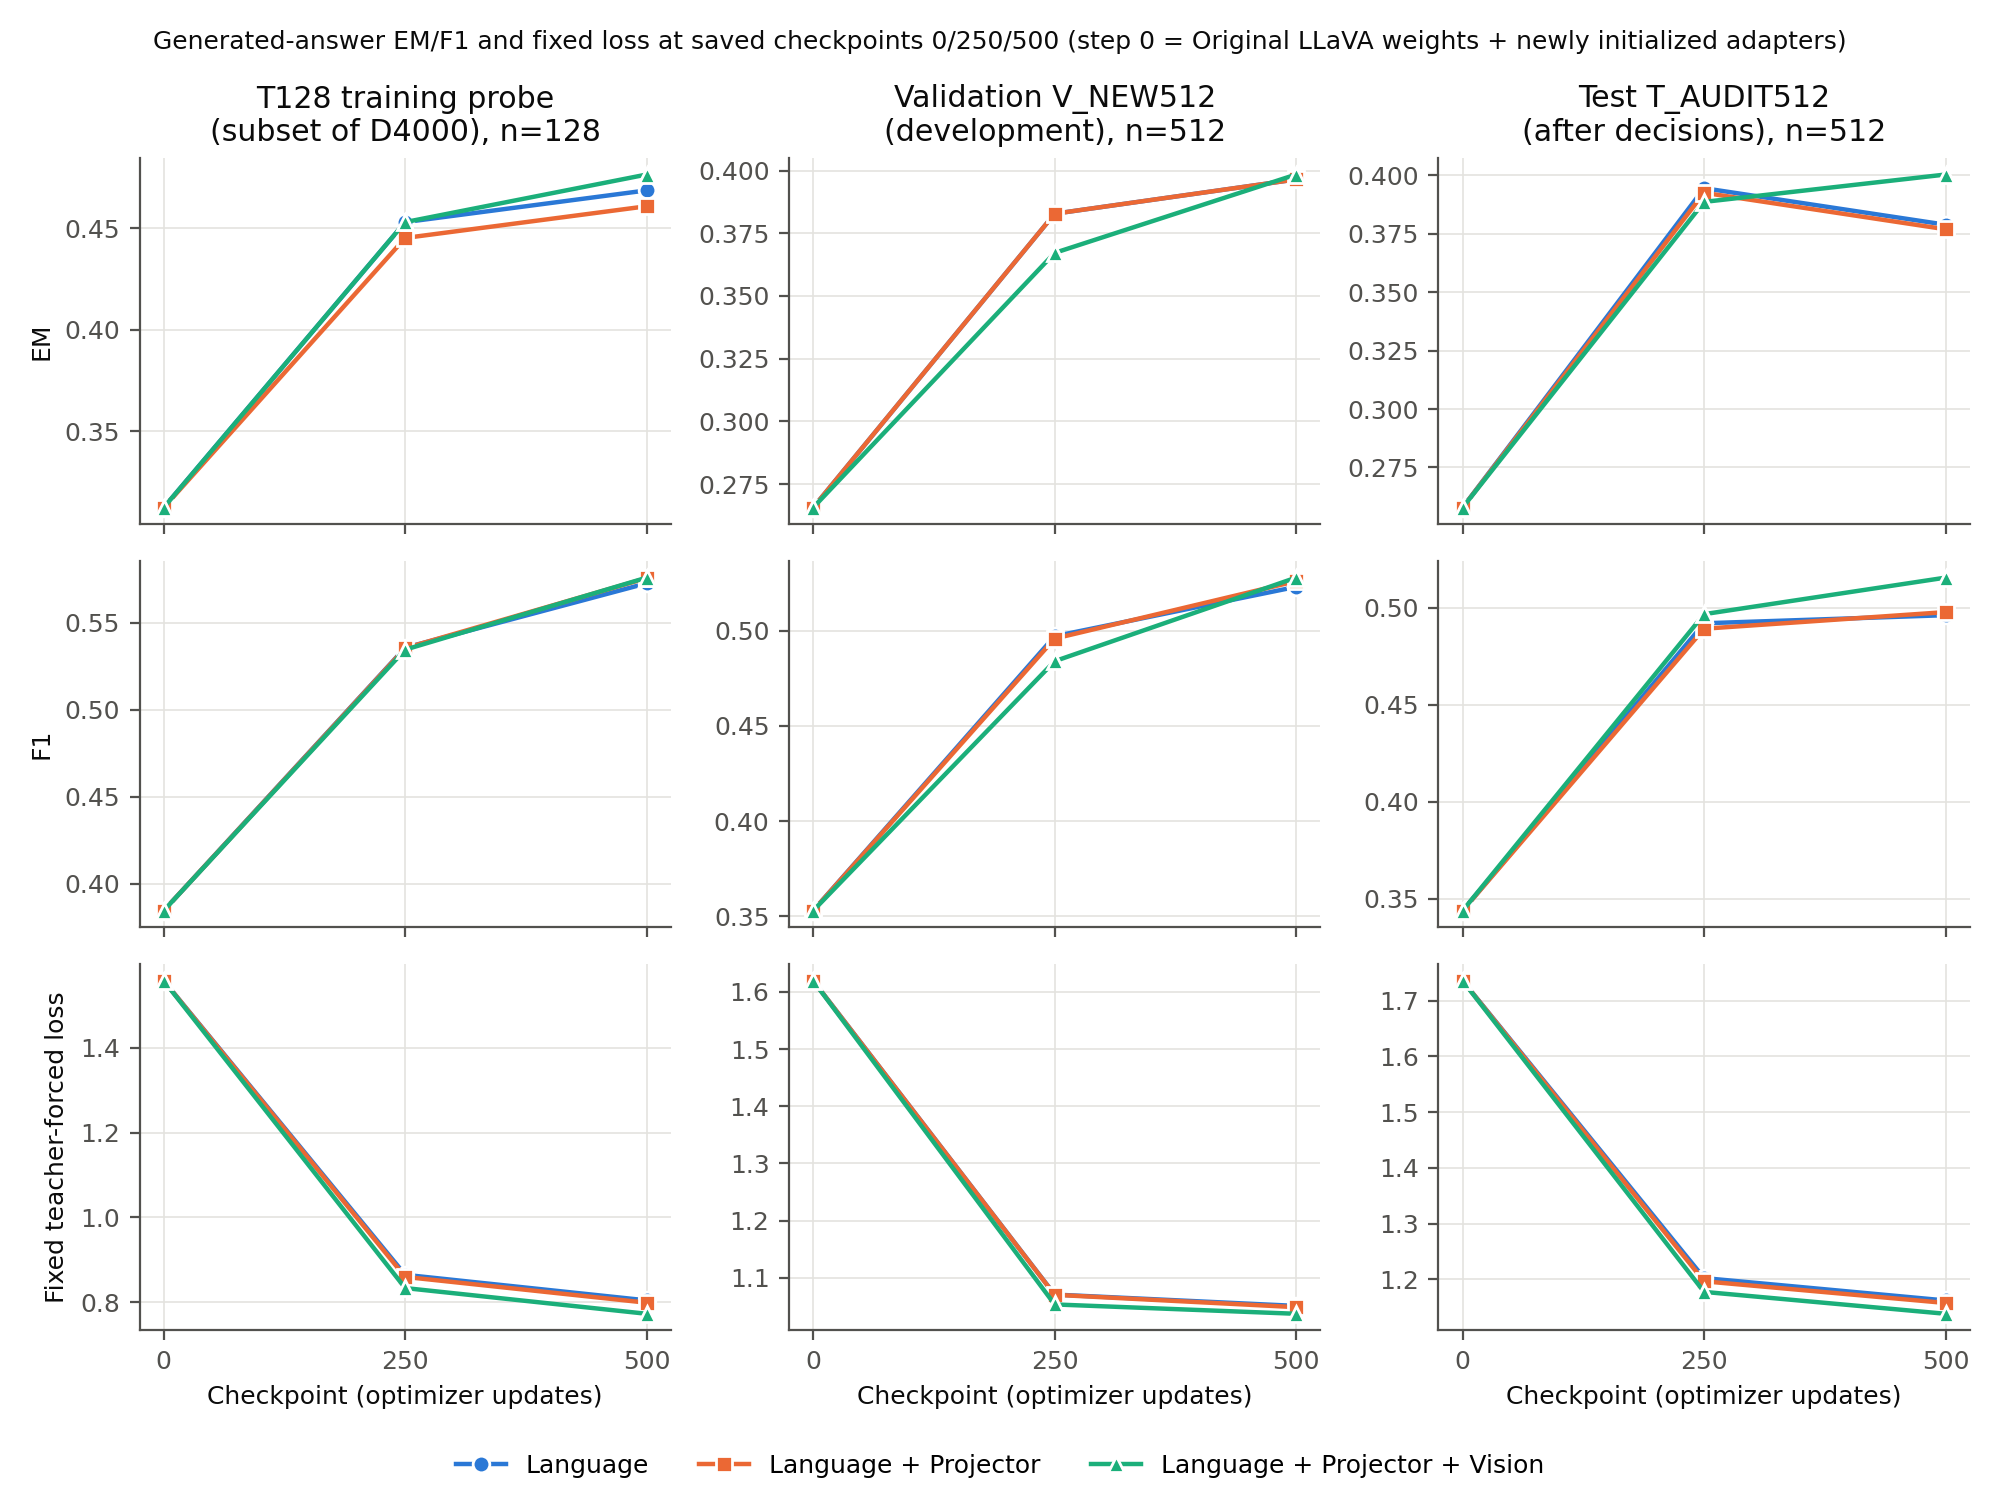
\includegraphics[width=0.82\linewidth]{src/fig_panel_curves.png}
  \caption{Generated-answer EM, F1 and fixed teacher-forced loss at checkpoints 0/250/500 for all scopes. Step 0 equals the Original model. Test curves (right) are descriptive and were computed after all decisions.}
  \label{fig:curves}
\end{figure*}

\begin{figure}[t]
  \centering
  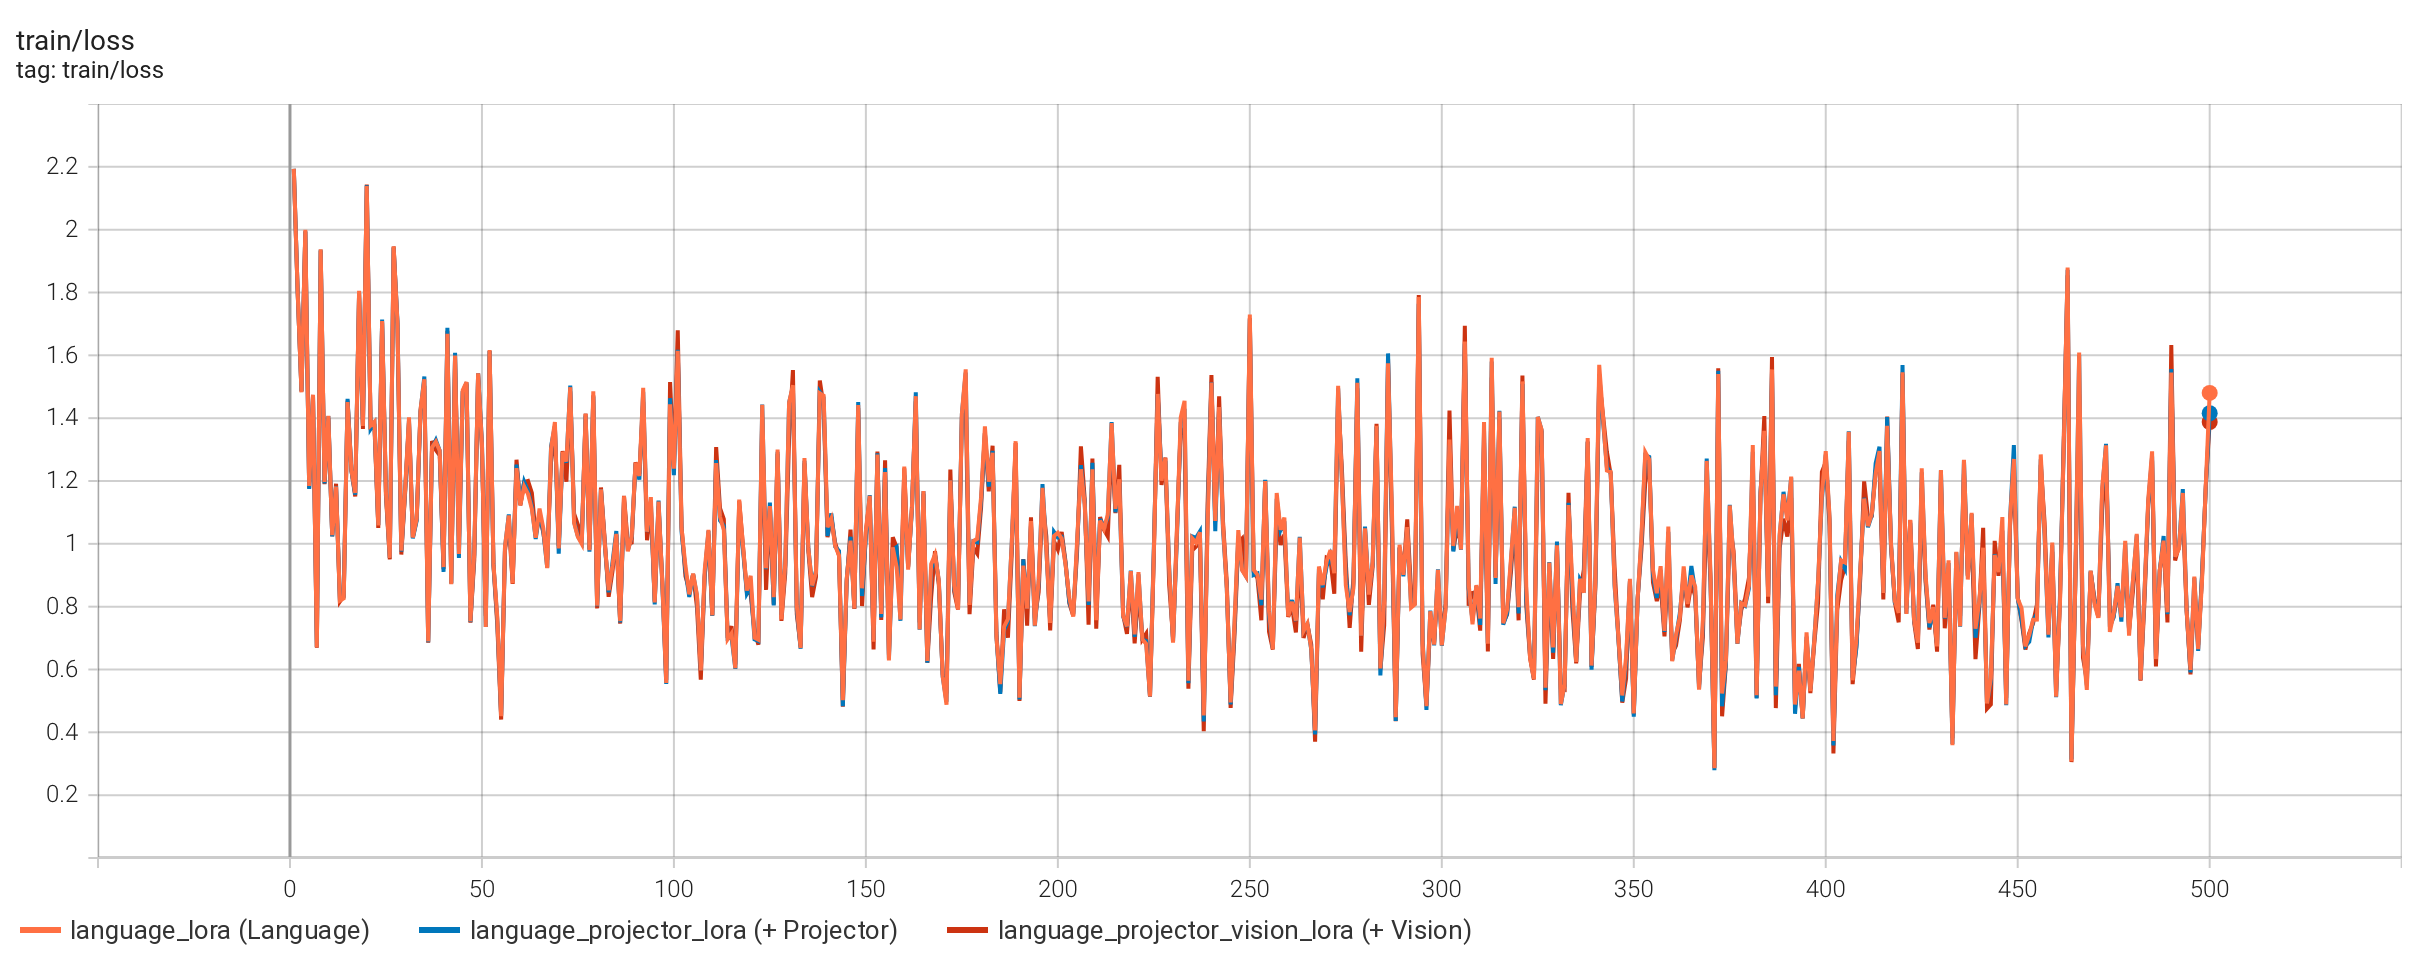
\includegraphics[width=\linewidth]{src/tb_train_loss_s0.png}\\[2pt]
  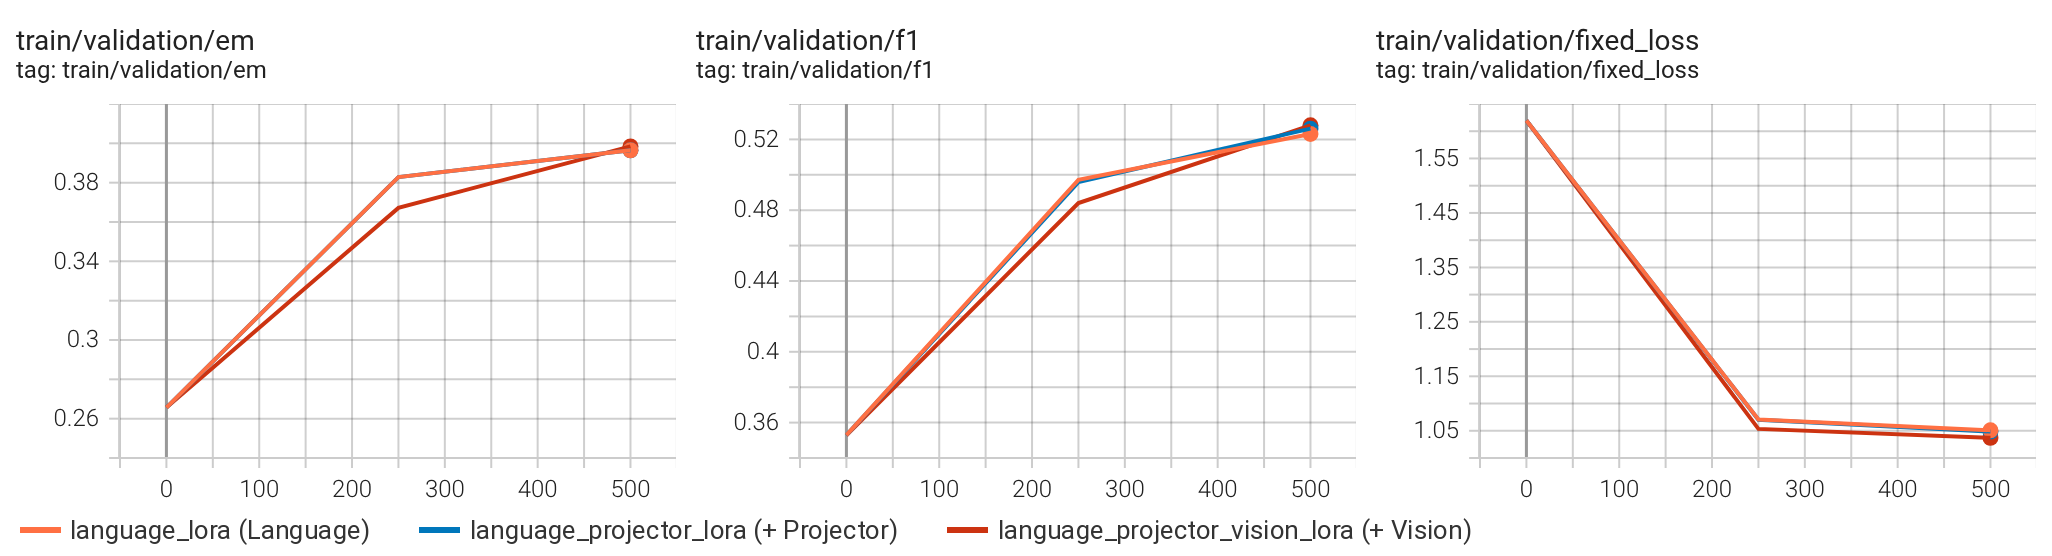
\includegraphics[width=\linewidth]{src/tb_validation_s0.png}
  \caption{TensorBoard views (smoothing 0, raw values). Top: online training loss per update (\texttt{train/loss}). Bottom: generated-answer EM, F1 and fixed teacher-forced loss on validation at checkpoints 0/250/500 (\texttt{train/validation/*}). TensorBoard colors differ from Fig.~\ref{fig:curves}: Language orange, + Projector blue, + Vision red.}
  \label{fig:loss}
\end{figure}

\paragraph{Curves.} The online loss (Fig.~\ref{fig:loss}, top) falls from 2.19 to about 0.8--1.0 within the first 100 updates, then plateaus without diverging; mean training loss is 0.998, 0.995 and 0.987 for the three scopes, and at TensorBoard's default smoothing of 0.6 (not shown) the same plateau is visible. It is noisy because each update averages only 8 examples. The fixed validation loss drops from 1.62 to 1.07 by step 250 and to 1.04--1.05 by step 500, and validation EM rises monotonically (Language: 26.6, 38.3, 39.7; Fig.~\ref{fig:curves}). Most of the gain is in the first half and there is no sign of overfitting within one epoch. On test, Language and + Projector peak in EM at step 250 (39.45 and 39.26) and dip at step 500 (37.89 and 37.70) while their F1 still rises; we report step 500 as prescribed. The evaluation progress bar shows running EM/F1 means over the items scored so far; every number in this report comes from completed evaluation files.

\paragraph{What the extra components buy.} Projector LoRA adds 106K parameters and changes almost nothing (test EM $-0.2$, F1 $+0.2$), and its curves overlap Language's. Vision LoRA gives the largest gains over Language ($+2.2$ test EM, $+1.9$ F1) and the lowest fixed loss on every split (test 1.138 vs.\ 1.162 for Language and 1.158 for + Projector). With $n=512$, the standard error of EM is about $\sqrt{0.39\cdot0.61/512}\approx2.2$ points, and a paired McNemar test~\cite{mcnemar1947} gives $p=0.061$ (Language vs.\ + Vision; 20 items gained, 9 lost; 95\% bootstrap CI of $\Delta$EM $[+0.2, +4.3]$ points) and $p=0.036$ against + Projector, neither significant after Holm correction over our six comparisons. With one seed, we therefore read the vision gain as small and not significant.

\paragraph{Abstention.} On test, 53 of 512 items have \noans{} as a reference answer. The Original model never abstains (0/512). After tuning, the three scopes abstain on 60/59/63 items, but only 20 of these are correct, giving \noans{} precision 0.33/0.34/0.32 and recall 0.38 for all three. Fine-tuning thus teaches the model to abstain, but false abstentions (40/39/43) outnumber correct ones, and 33 items with a \noans{} reference are still answered.

\paragraph{Cost.} Tab.~\ref{tab:cost} reports measured time and memory. Vision LoRA adds 2\% training time and negligible memory (+6\,MiB reserved). Evaluation (all checkpoints and splits) takes longer than training. The Torch peaks come from the full runs; the owned-process VRAM (\texttt{nvidia-smi}, filtered by our PID) was recorded in separate 10-update runs and includes the CUDA context.

\begin{table}[t]
  \centering
  \small
  \setlength{\tabcolsep}{4pt}
  \begin{tabular}{lrrr}
    \toprule
    & Language & + Proj. & + Vision \\
    \midrule
    Training (s)                   & 2,228.5 & 2,234.7 & 2,273.2 \\
    Evaluation (s)                 & 3,462.1 & 3,445.0 & 3,462.4 \\
    Total wall time (s)            & 5,711.1 & 5,698.6 & 5,755.0 \\
    Torch peak alloc.\ (GiB)       & 6.456 & 6.456 & 6.456 \\
    Torch peak reserved (GiB)      & 6.715 & 6.717 & 6.721 \\
    Process VRAM, 10 upd.\ (MiB)   & 7,166 & 7,168 & 7,170 \\
    \bottomrule
  \end{tabular}
  \caption{Measured cost per scope. Evaluating the Original model takes 272.5\,s (val), 274.9\,s (test) and 2,122.8\,s (D4000).}
  \label{tab:cost}
\end{table}

\paragraph{Benchmark examples.} Table~\ref{tab:cases} shows three test cases. On 000154 no zodiac sign is selected, yet the Original model names one (``Cancer''), while all three scopes correctly abstain. On 000765 the same learned abstention backfires: the waiting time is stated on screen and the Original answers correctly, but all three scopes decline, an instance of the 39--43 false abstentions above. On 000150 every model fails to match January 24 to its weekday column; the Original answers ``Monday'' and all three scopes ``Wednesday'', one day off on either side, so fine-tuning changes the answer but not the reading of the calendar grid.

\begin{table*}[t]
  \centering
  \footnotesize
  \setlength{\tabcolsep}{3pt}
  \begin{tabular}{p{1.9cm}p{4.2cm}lllll}
    \toprule
    Case (ID) & Question & Gold & Original & Language & + Projector & + Vision \\
    \midrule
    Correct (000154) & What is the selected zodiac sign? & \noans & \bad{Cancer} & \good{\noans} & \good{\noans} & \good{\noans} \\
    False (000765) & How much time will it take to receive the verification code? & 1 minute$^\ast$ & \good{1 minute} & \bad{\noans} & \bad{\noans} & \bad{\noans} \\
    Failure (000150) & What day is it on January 24? & Tuesday & \bad{Monday} & \bad{Wednesday} & \bad{Wednesday} & \bad{Wednesday} \\
    \bottomrule
  \end{tabular}
  \caption{Three ScreenQA test cases (screenshots \texttt{images/1049.jpg}, \texttt{6264.jpg}, \texttt{1019.jpg}); answers in \good{green} are correct, in \bad{red} wrong. $^\ast$One of six references, \eg ``up to 1 minute''; Tuesday also accepts ``Tue''.}
  \label{tab:cases}
\end{table*}
% ============================================================================ %
%                       4. TRANSFER TO PERSONAL IMAGES                         %
% ============================================================================ %

\section{Transfer to Personal Images}
\label{sec:transfer}

We rerun all ten personal questions, including the six screenshot questions, on the four models with the fixed best-effort prompt, which forbids declining (\emph{``\ldots You must answer every question. If you are uncertain \ldots make your best estimate \ldots Output only your best answer.''}). Tab.~\ref{tab:transfer} lists the answers.

\begin{table}[t]
  \centering
  \footnotesize
  \setlength{\tabcolsep}{4pt}
  \begin{tabular}{lllll}
    \toprule
    ID & Fig. & Expected & Original & All three LoRA scopes \\
    \midrule
    01-q1 & \ref{fig:own}a & 1          & \bad{10}          & \good{1} \\
    01-q2 & \ref{fig:own}a & Chrome     & \good{Chrome}     & \bad{``Chinese''} \\
    02-q1 & \ref{fig:own}b & McDonald's & \good{Mcdonald's} & \good{Mcdonald's} \\
    02-q2 & \ref{fig:own}b & 370        & \bad{300}         & \bad{300} \\
    03-q1 & \ref{fig:own}c & maths.cure & \bad{Math Cure}   & \bad{Maths Cure} \\
    03-q2 & \ref{fig:own}c & No         & \bad{Yes}         & \good{no} \\
    04-q1 & \ref{fig:own}d & 3          & \good{3}          & \good{3} \\
    04-q2 & \ref{fig:own}d & Yellow     & \good{Yellow}     & \good{yellow} \\
    05-q1 & \ref{fig:own}e & Right      & \good{Right}      & \good{right} \\
    05-q2 & \ref{fig:own}e & 2          & \good{2}          & \bad{3} \\
    \bottomrule
  \end{tabular}
  \caption{Best-effort answers on the personal benchmark. Language, + Projector and + Vision give identical answers on all ten questions, so they share one column. Answers in \good{green} are correct, in \bad{red} wrong.}
  \label{tab:transfer}
\end{table}

\paragraph{Target-task gains do not carry over.} The three scopes give the same answer on all ten questions, so every change comes from the language LoRA; the extra projector and vision capacity that helped slightly on ScreenQA has no visible effect here. Accuracy stays at 6/10 (two gained, two lost). Ten questions cannot establish general improvement or degradation, but they show that a 12-point benchmark gain does not imply better behavior on out-of-distribution screenshots.

\paragraph{01-q2 (right$\to$wrong): format transfer.} The tuned models answer \emph{``Chinese''} with quotation marks. ScreenQA answers often quote UI text, so the LoRA seems to have shifted the model from naming an icon to reading a label, and it reads an unrelated token near the dock. The same shift shows in the lowercase ``no'', ``yellow'' and ``right'', which match ScreenQA's answer style.

\paragraph{02-q2 (wrong$\to$wrong): perception, not format.} All models still answer 300 instead of 370. Fine-tuning taught the answer format but not to read the small balance next to the large, salient reward cost; since Qwen2.5-VL reads ``370'' from the same 336\,px input (Sec.~\ref{sec:judge}), the limit lies in LLaVA's visual encoding rather than in the pixels. 03-q1 is similar: the tuned models read the logo more closely (``Maths Cure'' instead of ``Math Cure'') but still not the exact handle.

\paragraph{03-q2 and 01-q1 (wrong$\to$right): learned UI state or shifted prior?} The tuned models now say the account is not followed and count one ball above the line. Both match ScreenQA's domain of on-screen state and objects. With one question each, we cannot tell whether the model learned button semantics or merely shifted toward short ``no'' and small-number answers; 05-q2 (two salads counted as three) argues against a general counting improvement. Prompt wording also matters: under the benchmark prompt the Original answers 03-q1 ``Maths Cure'', here ``Math Cure''.

% ============================================================================ %
%            5. BUILDING AN LVLM, LIMITATIONS AND CONCLUSION                   %
% ============================================================================ %

\section{Building an LVLM, Limitations and Conclusion}
\label{sec:build}

\subsection{Building Our Own LVLM}

\paragraph{Model and training.} We combine the frozen CLIP ViT-L/14-336 (303.5M parameters) with Qwen2.5-0.5B-Instruct (494.0M) through a two-layer GELU MLP adapter (1024$\to$896$\to$896, 1.72M parameters), as in LLaVA-1.5~\cite{liu2023improvedllava}. Tab.~\ref{tab:aplus} lists the settings; we use seed 42, no weight decay and gradient clip 1.0, and no samples were skipped. The recipe follows LLaVA-1.5 except for three instruction epochs, as in the original LLaVA. The alignment loss falls from 6.26 to 3.10. The instruction-tuning loss falls from 2.35 to 1.17 and drops abruptly at each epoch boundary ($\approx$1.40$\to$1.29 and 1.26$\to$1.16) while staying flat within each epoch, the usual sign that the model starts to memorize examples it has already seen.

\begin{table}[t]
  \centering
  \footnotesize
  \setlength{\tabcolsep}{3pt}
  \begin{tabular}{lll}
    \toprule
    & Stage 1: alignment & Stage 2: instruction \\
    \midrule
    Data            & CC3M-595K (full) & Instruct-150K + COCO \\
    Trainable       & adapter (1.7M) & adapter + LLM (495.8M) \\
    Epochs / steps  & 1 / 2,325 & 3 / 3,696 \\
    Eff.\ batch     & $8\times32=256$ & $4\times32=128$ \\
    LR / schedule   & $10^{-3}$, 3\% warmup, cosine & $2\times10^{-5}$, 3\% warmup, cosine \\
    Max length      & 1,024 & 2,048 (grad.\ ckpt.) \\
    Time / peak mem.& 275.9\,min / 8.40\,GB & 593.4\,min / 13.39\,GB \\
    \bottomrule
  \end{tabular}
  \caption{Training settings of our own LVLM; the vision encoder is frozen throughout.}
  \label{tab:aplus}
\end{table}

\begin{table*}[t]
  \centering
  \footnotesize
  \begin{tabular}{lp{0.42\linewidth}p{0.42\linewidth}}
    \toprule
    Stage & 02-q1 (Fig.~\ref{fig:own}b): Which company's app is this? [McDonald's] & 02-q2 (Fig.~\ref{fig:own}b): How many points do I have left? [370] \\
    \midrule
    Untrained (random adapter) & ``This is a reference to the company `The Company' (also known as `The Company' or `The Company Inc.')\ldots'' & ``I'm sorry, but I can't answer this question. This appears to be a multiple-choice question about music\ldots'' \\
    After alignment & ``the app is a mobile app that allows users to scan the code on their phone and pay for their purchases .'' & ``the points system is a way to reward customers for their loyalty .'' \\
    After instruction tuning & ``This image shows a McDonald's app, which is an app for ordering food and beverages from McDonald's restaurants.'' & ``You have 20 points left.'' \\
    \bottomrule
  \end{tabular}
  \caption{Our LVLM before training, after modality alignment and after instruction tuning (final checkpoint).}
  \label{tab:stages}
\end{table*}

\paragraph{Trends across stages (Tab.~\ref{tab:stages}).} \emph{Untrained}, the model cannot see the image: the random adapter turns visual tokens into noise, so it answers from text alone, inventing a company or treating the question as a quiz. \emph{After alignment} it does see the image: its captions are grounded (a payment app, a loyalty program; elsewhere a baseball pitcher and ``a bowl of soup with a salad''), but it ignores the question and writes in CC3M caption style, lowercase with a space before the period, exactly what stage 1 trains. \emph{After instruction tuning} it answers in the question's format and gets coarse semantic and spatial questions right (McDonald's, yellow jersey, soup on the right, three players), 4/10 in total. Text and counts remain out of reach: 370 becomes ``20'', \texttt{maths.cure} becomes an invented ``Ramon Men\'endez'', Chrome becomes ``a calculator'', and count answers oscillate between epochs (players 3$\to$2$\to$3, salads 3$\to$2$\to$3). Perception improves at each stage but only for coarse content; the adapter alone grounds the model, while instruction following needs the LLM to be tuned, and the 0.5B LLM fills gaps with fluent fabrications.

\paragraph{Hypothesized improvements.} (i) An OCR-oriented vision encoder or higher input resolution with AnyRes-style tiling; Qwen2.5-VL reads text that LLaVA misses from the same 336\,px input (Sec.~\ref{sec:judge}), so the encoder and its training data likely matter more than resolution alone. (ii) OCR- and UI-heavy instruction data, which LLaVA-1.5 adds and LLaVA-Instruct-150K lacks. (iii) Negative and abstention examples, since every ``Am I following?'' answer is ``Yes''. (iv) A larger LLM, or LoRA on late vision blocks, which already helped slightly in Sec.~\ref{sec:ft}, to reduce fabrication and sharpen fine-grained perception.

\subsection{Limitations}

(i) Each scope was trained with one seed, so differences of about 2 EM points are within noise. (ii) The personal benchmark has only ten questions, and our labels involve judgment calls such as whether a base coach is a player. (iii) Both judges come from the same model family and may share biases, and Qwen ran with a 4-bit LLM, which may understate it. (iv) The owned-process VRAM was recorded in separate 10-update runs, not the 500-update runs. (v) Our LVLM was evaluated only qualitatively on ten questions.

\subsection{Conclusion}

LLaVA-1.5-7B handles photo semantics but not small screen text. An LLM judge is order-stable yet can override human labels through its own visual errors. On ScreenQA Short a language LoRA provides most of the gain (+12 test EM), while projector and vision LoRA add little measurable improvement; the transfer to our own screenshots mixes gains and regressions and is identical across scopes. Building an LVLM from components clearly illustrates each stage of development—while feature alignment grants the model sight and instruction tuning enables it to respond, neither inherently teaches it to read.




%%%%%%%%% REFERENCES
{
    \small
    \bibliographystyle{ieeenat_fullname}
    \bibliography{main}
}

\end{document}